% ---------------------------------------------------------------------------
% Conference submission draft.
%
% COMPILE:  pdflatex main && bibtex main && pdflatex main && pdflatex main
%           (or drop the folder into Overleaf)
%
% BEFORE SUBMITTING:
%   1. Every \pending{...} must be replaced by a number backed by a run log or
%      removed. See SUBMISSION_CHECKLIST.md for the evidence register.
%   2. Swap the anonymous author block for the venue's required block, or keep
%      it for double-blind review.
%   3. Replace \documentclass{article} with the venue class file if required.
%   4. Check refs.bib entries marked % VERIFY.
% ---------------------------------------------------------------------------
\documentclass[10pt,twocolumn]{article}

\usepackage[margin=0.75in]{geometry}
\usepackage{mathptmx}
\usepackage[T1]{fontenc}
\usepackage[utf8]{inputenc}
\usepackage{amsmath,amssymb}
\usepackage{booktabs}
\usepackage{graphicx}
\usepackage{xcolor}
\usepackage{microtype}
\usepackage{tikz}
\usetikzlibrary{arrows.meta,positioning}
\usepackage[round]{natbib}
\usepackage[hidelinks]{hyperref}

% Quarantine macro for claims that are not yet backed by an artifact.
% A submission should contain zero of these.
\newcommand{\pending}[1]{\textcolor{red}{\textbf{[PENDING:} #1\textbf{]}}}

\title{\bfseries Synthesizability as a Design Constraint:\\
A Physics-Informed Generative Pipeline for\\
Auditable Early-Stage Molecular Design}

\author{Anonymous submission\\
Paper ID: \texttt{XXXX}\\
\textit{Do not distribute}
}

\date{}

\begin{document}
\maketitle

\begin{abstract}
Structure-based generative models now propose molecules at a rate no
medicinal-chemistry team can triage, yet most pipelines apply synthesizability
\emph{after} generation, as a filter on a candidate list. We describe a
pipeline in which route feasibility is treated as a constraint at the point of
design, and in which every prediction carries an explicit epistemic label
rather than an implicit score. The pipeline couples target-conditioned de novo
generation, structure-based docking with pose-level output, multi-pose
physics-based rescoring, independently cross-checked interaction
fingerprinting, a liability screen spanning ADMET, cardiac and hepatic
endpoints, a CYP450 interaction panel, and per-candidate retrosynthetic route
proposal from commercially available starting materials. We report a
retrospective pose-recovery case study on the Parkinson's disease kinase LRRK2
against the reference inhibitor MLi-2, and we set out the evaluation protocol
--- benchmark pose recovery, decoy discrimination, route-feasibility
adjudication, and ablation of the design constraints --- that a prospective
claim would require. We are explicit about what this work does not show: no
compound in this study has been synthesized or assayed, and pose recovery is
not evidence of prospective discovery. We contribute the architecture, a
reporting discipline for in-silico design claims, and a checklist that makes
the gap between a ranked docket and a validated hit auditable.
\end{abstract}

\section{Introduction}

Generative structure-based design has matured quickly: diffusion and
autoregressive models can now produce plausible ligands conditioned on a
protein pocket \citep{schneuing2024diffsbdd,peng2022pocket2mol,guan2023targetdiff}.
The bottleneck has moved downstream. A single campaign can emit thousands of
candidates, of which the overwhelming majority cannot be made on a useful
timescale, and a further fraction fail liabilities that are cheap to predict
and expensive to discover at the bench.

The common response is a filter chain: generate, dock, score, then discard
candidates that fail a synthesizability heuristic. This ordering has two
costs. First, it throws away generation budget on chemistry that was never
makeable, and the surviving set is a residue rather than a design. Second, and
more consequentially for the literature, it invites a reporting style in which
a docking score is presented as though it were a measurement. Docking scores
are not binding affinities \citep{trott2010vina}, and a redocked co-crystal
ligand recovery is a test of pose search, not of discovery.

This paper describes a pipeline built around the opposite ordering
(Section~\ref{sec:pipeline}): synthesizability and liability constraints are
evaluated during design, each candidate is emitted with its pose, contact map,
liability profile, and a proposed route as a single auditable record, and every
prediction carries a confidence label describing the strength of the evidence
behind it. We then report what we have and have not established
(Sections~\ref{sec:case} and~\ref{sec:evaluation}), and we state the protocol
under which a prospective claim could be made.

\paragraph{Contributions.}
\begin{enumerate}
\item An architecture in which route feasibility and liability screening are
generation-time constraints rather than post-hoc filters, and in which the unit
of output is an annotated candidate record rather than a ranked score
(Table~\ref{tab:modules}).
\item A multi-pose physics-based rescoring rule that selects among docked poses
using MM-GBSA support \citep{genheden2015mmpbsa}, with interaction fingerprints
independently confirmed by a second mapping method, so that a contact claim is
not the output of a single scorer.
\item An explicit confidence-labelling convention, applied per prediction,
whose purpose is to make the boundary between computed and measured quantities
legible to a reader who was not present for the campaign.
\item A retrospective pose-recovery case study on LRRK2 with the reference
inhibitor MLi-2 \citep{fell2015mli2}, reported with its protocol and its limits
(Section~\ref{sec:case}).
\item A reporting checklist (Appendix~\ref{app:checklist}) that separates
in-silico design claims from validated ones, intended to be reusable by other
groups reporting generative campaigns.
\end{enumerate}

We state at the outset, and repeat in Section~\ref{sec:limits}, that all
results in this paper are in-silico. No compound described here has been
synthesized or assayed.

\section{Related Work}

\paragraph{Structure-based generative models.}
Diffusion-based and autoregressive pocket-conditioned generators established
that chemically valid, pocket-complementary molecules can be sampled directly
\citep{schneuing2024diffsbdd,peng2022pocket2mol,guan2023targetdiff}. Their
evaluation, however, has centred on geometric and chemical validity rather than
on whether a proposed molecule can be made, and increasingly on whether the
predicted poses survive independent physical validity checks
\citep{buttenschoen2024posebusters}.

\paragraph{Docking, rescoring, and the score-as-measurement problem.}
Empirical scoring functions remain fast but weakly correlated with affinity
\citep{trott2010vina}; end-to-end learned pose predictors offer an alternative
without an explicit scoring function \citep{torng2019gnn}. End-point free-energy
methods such as MM-GBSA sit between docking and alchemical free energy in cost
and reliability \citep{genheden2015mmpbsa}. Our use of MM-GBSA is deliberately
narrow: it arbitrates between poses of the same ligand, where correlated errors
partially cancel, and we do not use it to rank different ligands.

\paragraph{Synthesizability and retrosynthesis.}
Synthesizability has been formalized as a learned property of proposed
molecules \citep{gao2020synthesizability} and operationalized through
retrosynthetic search over available building blocks. We treat the latter as a
feasibility oracle during design: a candidate whose route cannot be closed from
commercially available starting materials is deprioritized before it consumes
downstream scoring budget.

\paragraph{Liability prediction and its ceiling.}
Rule-based property filters remain useful summaries
\citep{lipinski1997,baell2010pains,bickerton2012qed}, and QSAR models for
absorption, toxicity, and CYP inhibition are standard. Their accuracy outside
the applicability domain of their training data is the central caveat, which is
why we attach confidence labels to liability predictions rather than treating
them as determinations.

\section{Pipeline}
\label{sec:pipeline}

\begin{figure*}[t]
\centering
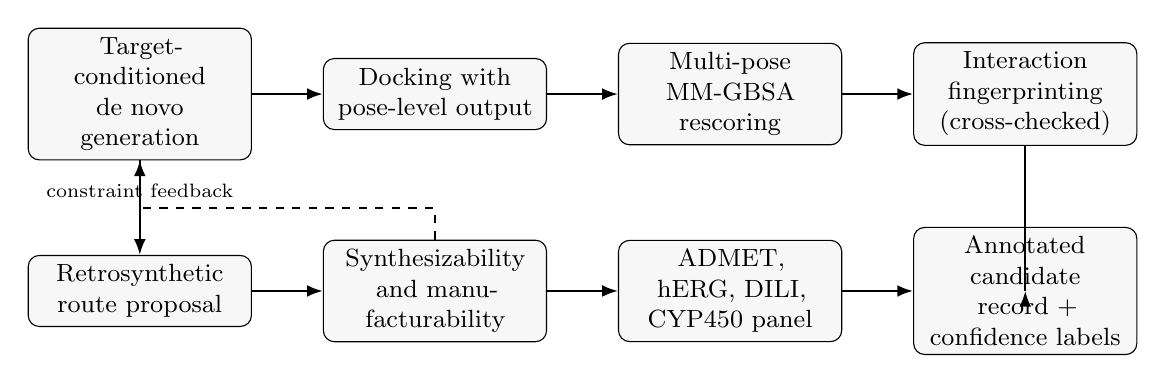
\begin{tikzpicture}[
  node distance=6mm and 9mm,
  box/.style={draw, rounded corners, align=center, font=\small,
              minimum height=9mm, text width=26mm, fill=black!3},
  group/.style={draw, dashed, rounded corners, inner sep=3mm},
  arr/.style={-{Latex[length=2mm]}, thick}
]
\node[box] (gen) {Target-conditioned\\de novo generation};
\node[box, right=of gen] (dock) {Docking with\\pose-level output};
\node[box, right=of dock] (rescore) {Multi-pose\\MM-GBSA rescoring};
\node[box, right=of rescore] (ifp) {Interaction\\fingerprinting\\(cross-checked)};

\node[box, below=12mm of gen] (route) {Retrosynthetic\\route proposal};
\node[box, right=of route] (synth) {Synthesizability\\and manufacturability};
\node[box, right=of synth] (admet) {ADMET, hERG, DILI,\\CYP450 panel};
\node[box, right=of admet] (record) {Annotated candidate\\record +\\confidence labels};

\draw[arr] (gen) -- (dock);
\draw[arr] (dock) -- (rescore);
\draw[arr] (rescore) -- (ifp);
\draw[arr] (gen) -- (route);
\draw[arr] (route) -- (synth);
\draw[arr] (synth) -- (admet);
\draw[arr] (admet) -- (record);
\draw[arr] (ifp) |- (record);
\draw[arr, dashed] (synth.north) -- ++(0,4mm) -| (gen.south)
  node[midway, above, font=\scriptsize] {constraint feedback};
\end{tikzpicture}
\caption{Design-time constraint ordering. Route feasibility and liability
screening run in the loop with generation (dashed feedback), rather than as a
filter applied to a finished candidate list. The unit of output is an annotated
record: structure, pose, contact map, liability profile, proposed route, and
per-prediction confidence labels.}
\label{fig:pipeline}
\end{figure*}

\subsection{Design principles}

Three rules govern the implementation.

\emph{(i) Constraint before scoring.} Any candidate that fails a
synthesizability or hard-liability constraint is deprioritized before it
consumes docking, rescoring, or liability compute. Generation budget is
therefore spent on chemistry that can plausibly be made.

\emph{(ii) One candidate, one record.} A candidate is never emitted as a bare
score. It is emitted with the pose it was scored in, the residue-level contacts
that pose makes, its liability profile, a proposed route, and the label of the
model that produced each field.

\emph{(iii) Nothing is presented as more certain than the evidence behind it.}
Each prediction carries an explicit confidence label distinguishing, for
example, a redocked reference ligand from a prospective proposal, or a
prediction inside a model's applicability domain from one outside it. This is
a design principle about reporting, not a claim about accuracy.

\subsection{Modules}

Table~\ref{tab:modules} lists the stages. The pipeline spans generation through
route proposal; module boundaries are deliberately coarse, because the
individually interesting question is not how many components exist but whether
the record a chemist receives is sufficient to decide what to do next.

\begin{table*}[t]
\centering
\small
\begin{tabular}{@{}p{4.6cm}p{11.2cm}@{}}
\toprule
\textbf{Stage} & \textbf{Output and role} \\
\midrule
Candidate generation & Novel structures generated against the target pocket,
not retrieved from a screening library. \\
Structure-based docking & Pose-level output; the pose, not only a score, is
retained for every candidate. \\
Physics-based rescoring & MM-GBSA across multiple docked poses per candidate;
the best-supported pose is selected rather than a single docking run being
trusted. \\
Interaction fingerprinting & Residue-level contacts, independently confirmed
by a second interaction-mapping method. \\
Potency modelling & QSAR potency estimate, labelled with its applicability
domain. \\
ADMET profiling & Per-candidate absorption, distribution, metabolism,
excretion and toxicity summary. \\
Safety and selectivity & Off-target receptor panel; cardiac (hERG) and hepatic
(DILI) liability. \\
Metabolic liability & CYP450 inhibition across 1A2, 2C9, 2C19, 2D6 and 3A4;
drug--drug interaction prediction built on that panel. \\
CNS exposure & Blood--brain barrier penetration model. \\
Metabolite identification & Predicted metabolites, with reactive and toxic
species flagged and bioactivation scored. \\
Manufacturability & Synthesizability and route-feasibility scoring. \\
Route proposal & Retrosynthetic routes from commercially available starting
materials, per candidate, for chemist adjudication. \\
Multi-target scoring & Candidates optimized against two or more pockets
simultaneously through the same safety panels. \\
Pose-confidence flagging & Indicates which poses are conformationally
reliable, weighted by pocket flexibility so that confidence reflects
target-side as well as ligand-side uncertainty. \\
\bottomrule
\end{tabular}
\caption{Pipeline stages. Every row is a computation, not a measurement. The
confidence convention of Section~\ref{sec:confidence} attaches to each.}
\label{tab:modules}
\end{table*}

\subsection{Multi-pose rescoring}
\label{sec:rescore}

For each candidate we retain the top docked poses and compute an end-point
binding estimate for each \citep{genheden2015mmpbsa}. Selection is by
best-supported pose, with a stability requirement: a candidate whose poses
disagree about the dominant interaction pattern is flagged rather than scored
on its most favourable pose. This is a variance-reduction device. It reduces
the influence of a single lucky docking run; it does not convert an end-point
estimate into a free energy.

\subsection{Independently cross-checked contacts}
\label{sec:contacts}

A contact claim is the part of a docket a chemist is most likely to act on, so
it is the part most dangerous to produce from one scorer. Each pose's contacts
are mapped by two methods, and a contact is reported only where they agree;
disagreements are surfaced as uncertainty in the record rather than resolved
silently in favour of the more flattering method.

\subsection{Synthesizability as a constraint}
\label{sec:synth}

Route proposal runs inside the design loop (Figure~\ref{fig:pipeline}, dashed
edge). A candidate whose route cannot be closed from commercially available
starting materials within the search budget is deprioritized before it reaches
the liability screen. We emphasize the scope of this claim: a route proposal
establishes that a plausible path exists from purchasable materials. It does
not establish yield, impurity profile, cost, or scalability, and it is not a
CMC assessment. Those are process-chemistry judgements outside the pipeline.

\subsection{Confidence labelling}
\label{sec:confidence}

Labels are assigned per prediction along two axes: \emph{evidence class}
(redocked reference ligand, retrospective benchmark, prospective proposal) and
\emph{domain position} (inside or outside the training distribution of the
model that produced the number). Downstream, a reader can therefore
distinguish, without consulting the campaign log, a pose recovered for a ligand
whose crystal structure is known from a pose proposed for a molecule that has
never been made.

\section{Retrospective Case Study: LRRK2 and MLi-2}
\label{sec:case}

\paragraph{Why this target.} LRRK2 is a Parkinson's disease kinase with a
well-characterized reference inhibitor, MLi-2 \citep{fell2015mli2}, whose
co-crystal structure supplies a ground-truth pose. Redocking a known ligand
tests pose search and scoring against a known answer.

\paragraph{Protocol.} The reference ligand is extracted from its co-crystal
structure, docked back into the prepared pocket, and evaluated on (i) heavy-atom
RMSD to the crystallographic pose, with a 2\,\AA{} success threshold, and (ii)
recovery of the hinge contacts reported for the complex (GLU1948, ALA1950).
Poses are additionally rescored by the multi-pose MM-GBSA rule of
Section~\ref{sec:rescore}.

\paragraph{Reported outcomes and their status.} Table~\ref{tab:status} lists
every quantitative claim associated with this case study alongside its
evidentiary status. Two figures in the source material conflict, and one has no
retained run log. We report the conflict rather than resolving it by
preference; the submission version of this paper will carry only reconciled
values, each traceable to a log file.

\begin{table*}[t]
\centering
\small
\begin{tabular}{@{}p{3.6cm}p{4.4cm}p{4.0cm}p{3.8cm}@{}}
\toprule
\textbf{Quantity} & \textbf{Reported value(s)} & \textbf{Status} & \textbf{What settles it} \\
\midrule
MLi-2 redock RMSD & Sub-2\,\AA{}; separately 2.9\,\AA{} $\rightarrow$
0.4\,\AA{} after rescoring & Conflicting & Retained docking and rescoring logs
with seed and receptor preparation \\
Docking score & $-9.5$ kcal\,mol$^{-1}$ & Unverified by artifact &
Scoring log from the stated configuration \\
Campaign runtime & 19 min; separately 7.46 h for a nine-target docket on one
GPU node & Conflicting & Timestamped job record; the two almost certainly
describe different configurations \\
Model inventory & 12+ validated; 18 trained; 24+ modules (different documents)
& Conflicting & Frozen manifest with versions and checkpoints \\
Route-feasibility check & Checked against known easy and hard marketed drugs
& Dataset, $n$ and result unrecorded & Re-run with the reference set named in
the protocol \\
Wet-lab validation & None & Absent & Would require synthesis and assay \\
Prospective discovery & None & Absent & Would require a prospective campaign \\
\bottomrule
\end{tabular}
\caption{Quantitative claims for the LRRK2 case study and their evidentiary
status at the time of writing. Rows marked conflicting or absent are removed
before submission unless reconciled.}
\label{tab:status}
\end{table*}

\paragraph{What this case does and does not show.} It shows that the pose-search
and rescoring stages can recover a known binding mode for a kinase with a
well-defined hinge interaction. It does not show that a novel molecule proposed
by the pipeline binds, is selective, is synthesizable in practice, or is
therapeutically useful. Redocking a known ligand is a necessary sanity check on
the front of the pipeline and is not evidence about its back end.

\section{What a Prospective Claim Would Require}
\label{sec:evaluation}

A single-case redock cannot support a generalization claim. We therefore
specify the evaluation we regard as adequate, and we distinguish it from what
this draft contains.

\paragraph{Pose recovery at scale.} A benchmark of co-crystal complexes, with
top-1 and top-5 success at 2\,\AA{}, reported per target family, and filtered
for physical validity of the predicted poses rather than RMSD alone
\citep{buttenschoen2024posebusters}.

\paragraph{Discrimination, not score.} Paired active/decoy sets, evaluated by
ranking metrics rather than by the magnitude of any single score, to test
whether rescoring orders candidates correctly rather than merely producing
plausible numbers.

\paragraph{Route feasibility with human adjudication.} A named reference set of
molecules spanning easy and hard syntheses, with routes judged by chemists
against a stated rubric, reporting inter-rater agreement. A synthesizability
score without an adjudication protocol is a self-assessment.

\paragraph{Ablations of the design constraints.} Generation with and without
the synthesizability constraint, to test the central architectural claim: that
constraining at design time yields a candidate set that is not merely a filtered
subset of the unconstrained one. Multi-pose versus single-pose rescoring, to
isolate the variance-reduction contribution. Cross-checked versus
single-method contacts, to quantify how often the two methods disagree.

\paragraph{Prospective validation.} The only claim that would justify the word
\emph{discovery}: candidates selected by the pipeline, synthesized, and assayed,
with the selection predating the assay. Until that exists, the appropriate
register for this work is methodological.

\section{Limitations}
\label{sec:limits}

\emph{No wet-lab validation.} No compound described here has been synthesized
or tested. Every result is computational.

\emph{No affinity claim from docking.} Docking and end-point rescoring are used
to select poses, not to rank molecules by binding strength. Reported scores
should not be read as affinities.

\emph{Route proposals are proposals.} A closed route from purchasable starting
materials demonstrates plausibility, not yield, purity, cost, or scalability.

\emph{Single-case retrospective.} The case study covers one target and one
reference ligand, chosen because a ground-truth pose exists. It is a sanity
check, not a benchmark.

\emph{Applicability domain.} Learned liability and potency models are reliable
only within the chemistry they were trained on; predictions outside that domain
carry the corresponding label and should be treated as hypotheses.

\emph{Compute reproducibility.} Configurations reported in earlier internal
documents disagree on runtime; this draft therefore makes no performance claim
until the configurations are reconciled and logged.

\section{Reproducibility and Availability}

The submission version will report, for every table entry, the command, seed,
receptor preparation, model checkpoint identifier, and hardware used to produce
it, and will state which artifacts are released with the paper. Where an
artifact cannot be released, the reason will be given rather than the row
silently omitted.

\section{Conclusion}

Treating synthesizability as a constraint at design time, and attaching an
explicit evidence label to every prediction, changes what a generative
campaign hands to a chemist: not a ranked list of scores, but a set of
candidates whose provenance is legible. We have described such a pipeline, set
out a retrospective case study with its limits stated, and specified the
evaluation that would be needed before any prospective claim could be made.
The most useful contribution at this stage may be the discipline of the
reporting rather than the numbers: a ranked docket and a validated hit are
different objects, and conflating them is the failure mode this work is built
to prevent.

\appendix
\section{Reporting checklist}
\label{app:checklist}

Each item should be answerable from the paper or its supplement without
contacting the authors.

\begin{enumerate}
\item Is every number in the results traceable to a named artifact (log,
      checkpoint, dataset version)?
\item Are conflicting internal figures reconciled, with the discarded value and
      the reason stated?
\item Is the distinction between redocked reference ligand, retrospective
      benchmark, and prospective proposal explicit at the point of each claim?
\item Is the applicability domain of each learned model stated, and are
      out-of-domain predictions labelled?
\item Are route proposals accompanied by an adjudication protocol and by
      agreement statistics?
\item Is hardware, runtime, seed and checkpoint reported for every experiment?
\item Is it stated, in the abstract and not only in a limitations section, that
      no wet-lab validation exists?
\item Are data and code availability statements specific about what is
      released, and why anything withheld is withheld?
\item Has all internal commercial material been excluded from the submission,
      including partner names, target identities under agreement, and
      non-public commercial strategy?
\end{enumerate}

\bibliographystyle{plainnat}
\bibliography{refs}

\end{document}
